\paragraph{Registrazione}

\label{Diagramma di Sequenza - Registrazione}

\begin{figure}[ht]
	\centering
	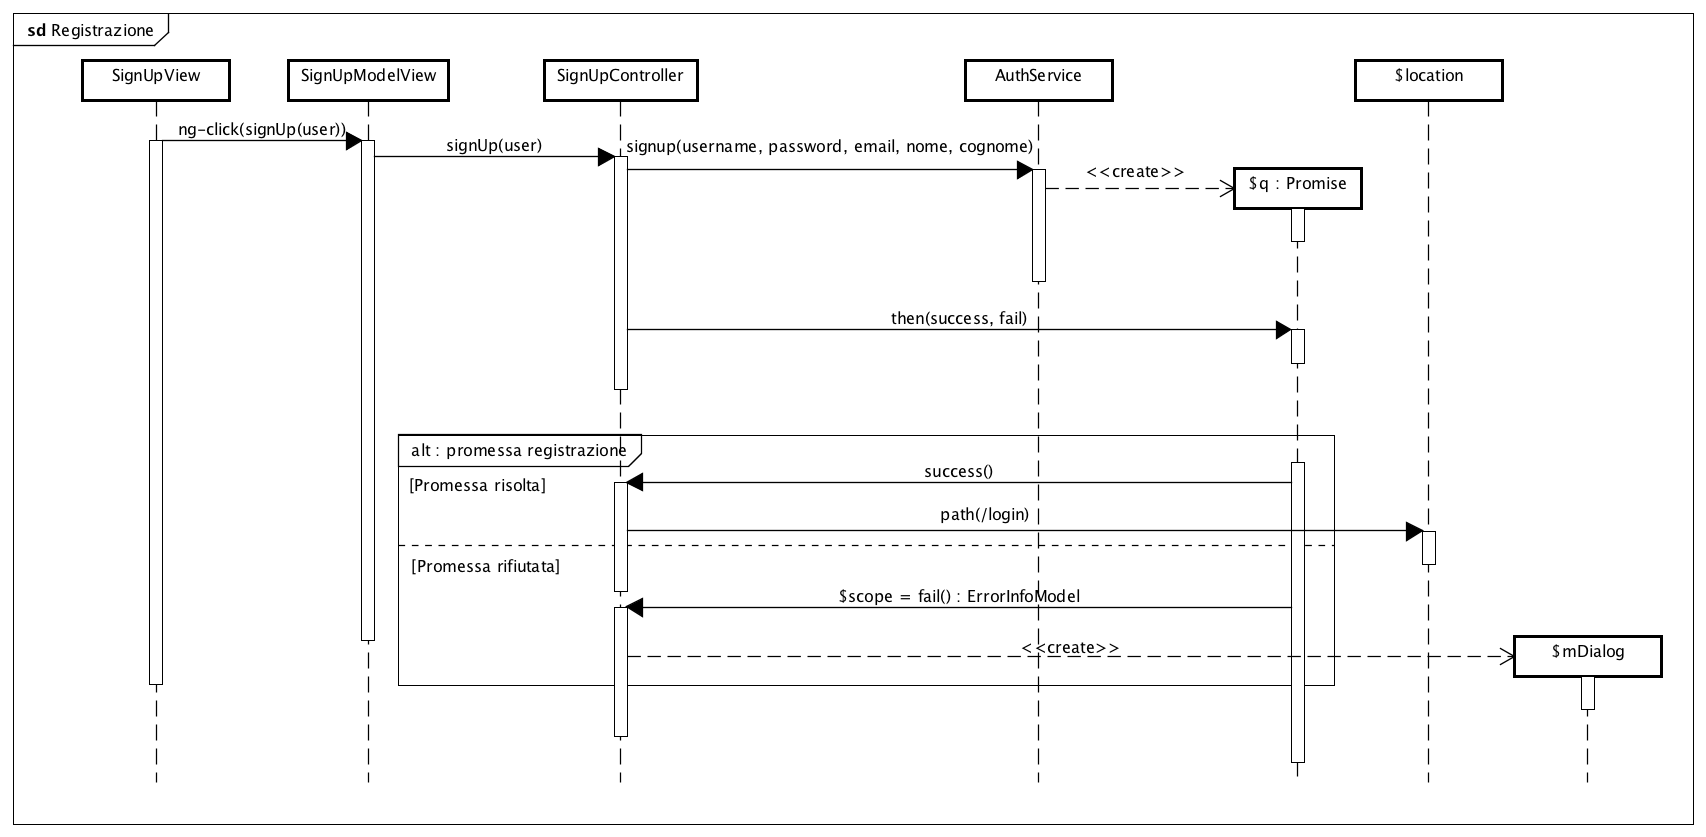
\includegraphics[scale=0.4,keepaspectratio]{UML/DiagrammiDiSequenza/Front-end/SignUp.png}
	\caption{Diagramma di Sequenza - Registrazione}
\end{figure} \FloatBarrier

L'utente dopo aver inserito tutti i campi richiesti, può effettuare la registrazione avviando l'evento associato al bottone presente in \texttt{SignUpView}. Il \texttt{SignUpController} gestisce l'evento chiamando il metodo \texttt{signup} dell'\texttt{AuthService}, il quale restituisce una promessa. Se la promessa viene soddisfatta l'utente viene reindirizzato alla pagina di login, altrimenti verrà restituito un oggetto di tipo \texttt{ErrorInfoModel} e mostrato a video mediante \texttt{\$mdDialog}.